\newpage
\section{Podręcznik użytkownika}  %6
%Opis jak używać programu. Mogą być z zrzut ekranu razem z opisem. 
\begin{figure}[!hbt]
		\begin{center}
			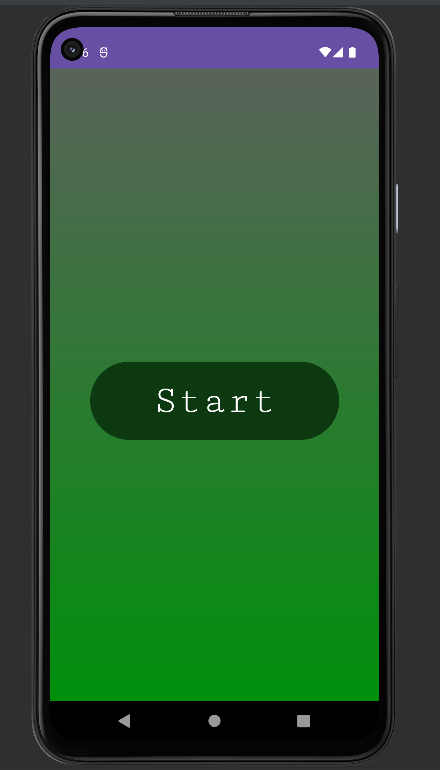
\includegraphics[width=5 cm]{rys/pu/1.png}
			\caption{Start}
			\label{rys:start}
		\end{center}
	\end{figure}
 \hspace{0,60 cm} Grafika \ref{rys:start} przedstawia wygląd po uruchomieniu aplikacji. Wita nas napis "Start", w którego należy nacisnąć aby przejść dalej.
\begin{figure}[!hbt]
		\begin{center}
			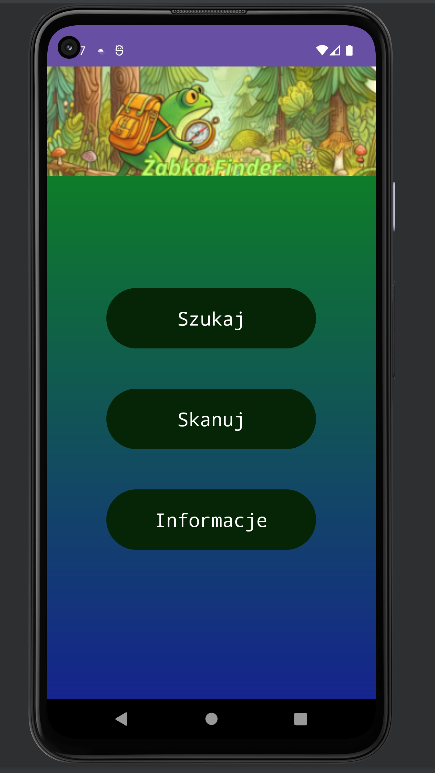
\includegraphics[width=5 cm]{rys/pu/2 .png}
			\caption{Strona główna}
			\label{rys:strona-glowna}
		\end{center}
	\end{figure}
 
\hspace{0,60 cm} Rysunek \ref{rys:strona-glowna} przedstawia menu główne aplikacji, z którego przechodzimy w różne funkcjonalności aplikacji. Po wciśnięciu przycisku "Szukaj", efekt pokazuje grafika \ref{rys:szukaj}. Wciśnięcie przycisku "Skanuj", otwiera aparat i pozwala zeskanować kod QR. Przedstawiają to rysunki \ref{rys:skanuj} oraz \ref{rys:komunikat}. Po wybraniu przycisku "Informacje", trafimy na kolejną podstronę, przedstawia to rysunek \ref{rys:podstrona}.
\begin{figure}[!hbt]
		\begin{center}
			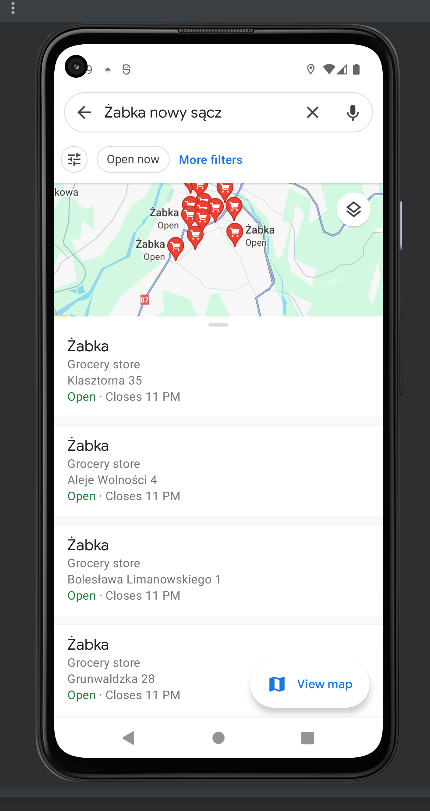
\includegraphics[width=5 cm]{rys/pu/10.png}
			\caption{Szukaj}
			\label{rys:szukaj}
		\end{center}
	\end{figure}
 
 \begin{figure}[!hbt]
		\begin{center}
			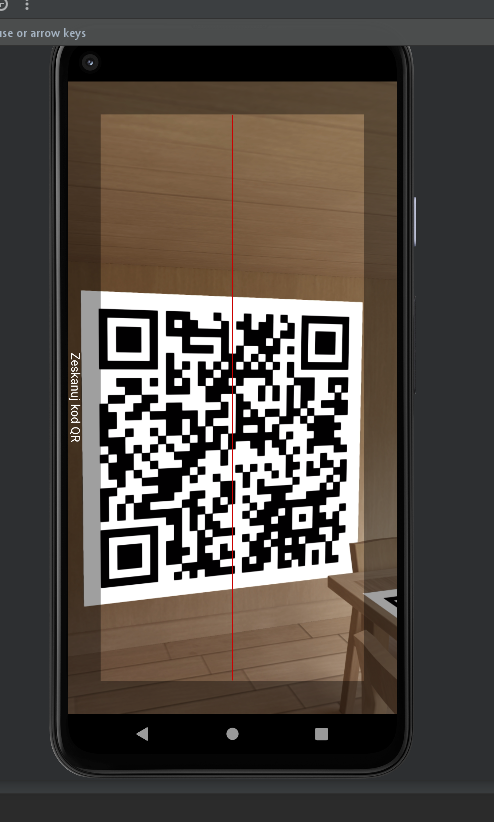
\includegraphics[width=5 cm]{rys/pu/8.png}
			\caption{Skanuj}
			\label{rys:skanuj}
		\end{center}
	\end{figure}
 
 \begin{figure}[!hbt]
		\begin{center}
			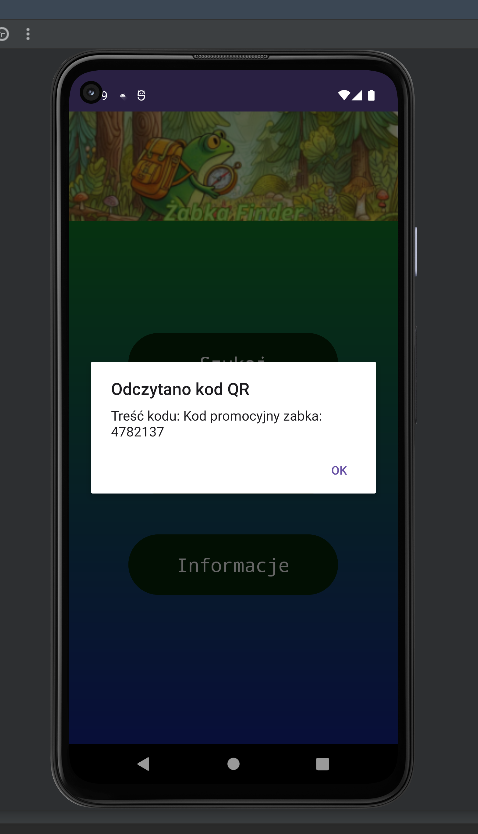
\includegraphics[width=4.9 cm]{rys/pu/9.png}
			\caption{Komunikat po skanowaniu}
			\label{rys:komunikat}
		\end{center}
	\end{figure}
 
 \newpage
  \hspace{0,60 cm} Jak pokazano na grafice \ref{rys:podstrona}, na tej podstronie mamy 4 funkcjonalne przyciski. Naciskając "O nas", użytkownik dostaje informacje o autorach aplikacji. Przedstawia to grafika \ref{rys:o nas}. Po naciśnięciu "Wersja" otrzymujemy informacje, czy wersja aplikacji jest aktualna (rysunki \ref{rys:wersja} ; \ref{rys:wersja powiadomienie}). Przycisk "Opcje" umożliwia użytkownikowi wprowadzenie imienia (rysunki \ref{rys:zmiana imienia} ; \ref{rys:zmiana imienia-powiadomienie}). Przycisk "Powrót" przekierowuje z powrotem do strony głównej.
  \begin{figure}[!hbt]
		\begin{center}
			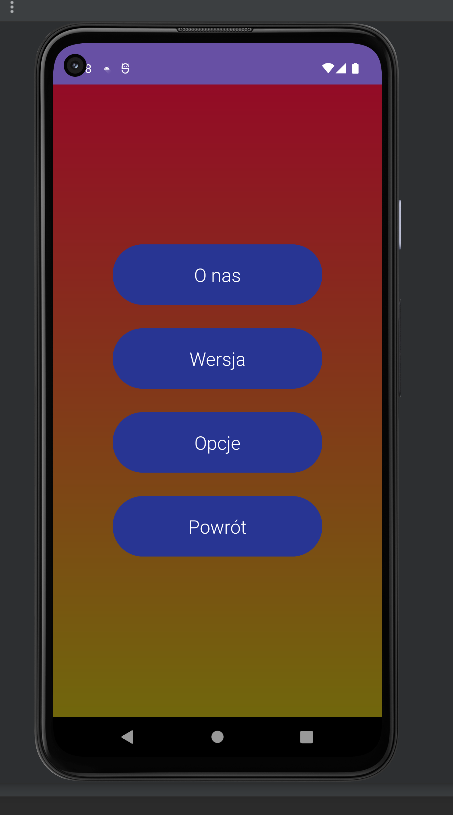
\includegraphics[width=5 cm]{rys/pu/7.png}
			\caption{Podstrona}
			\label{rys:podstrona}
		\end{center}
	\end{figure}

    \newpage
   \begin{figure}[!hbt]
		\begin{center}
			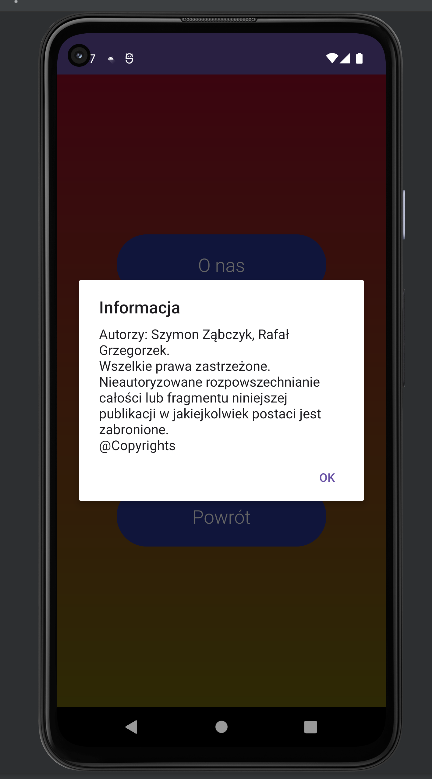
\includegraphics[width=5 cm]{rys/pu/4.png}
			\caption{O nas}
			\label{rys:o nas}
		\end{center}
	\end{figure}

   \begin{figure}[!hbt]
		\begin{center}
			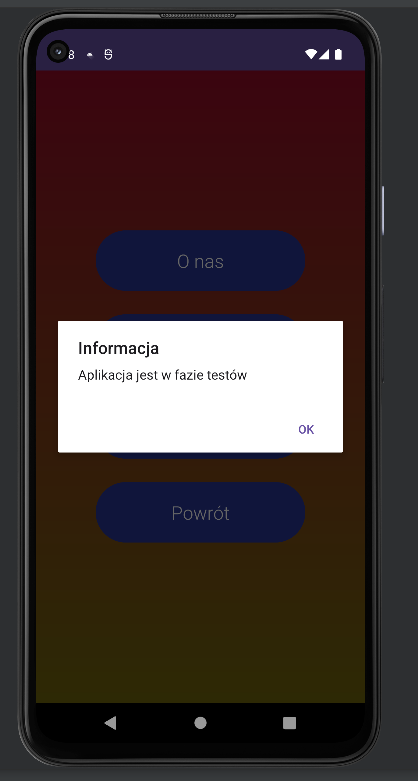
\includegraphics[width=5 cm]{rys/pu/5.png}
			\caption{Wersja}
			\label{rys:wersja}
		\end{center}
	\end{figure}

   \begin{figure}[!hbt]
		\begin{center}
			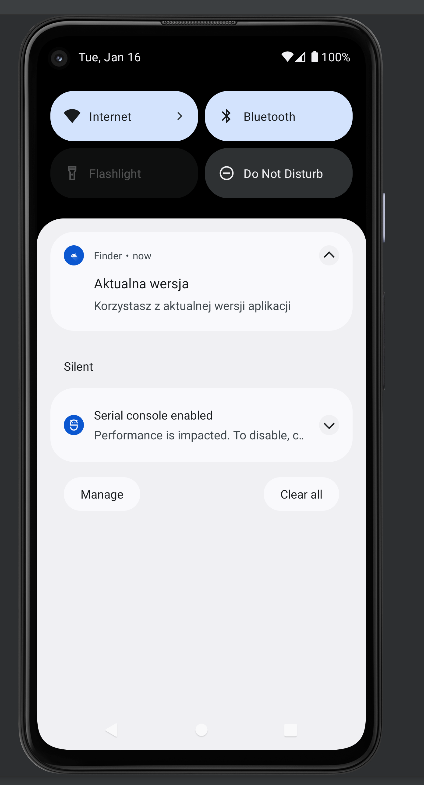
\includegraphics[width=5 cm]{rys/pu/11.png}
			\caption{Wersja powiadomienie}
			\label{rys:wersja powiadomienie}
		\end{center}
	\end{figure}

 \begin{figure}[!hbt]
		\begin{center}
			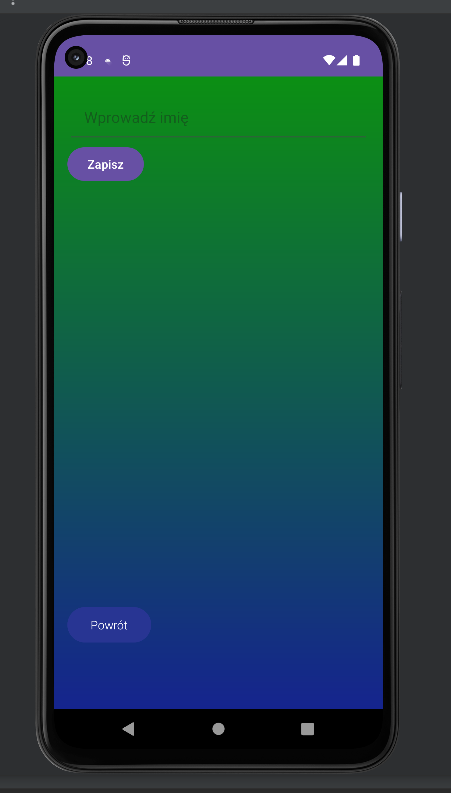
\includegraphics[width=6 cm]{rys/pu/6.png}
			\caption{Zmiana imienia}
			\label{rys:zmiana imienia}
		\end{center}
	\end{figure}

\begin{figure}[!hbt]
		\begin{center}
			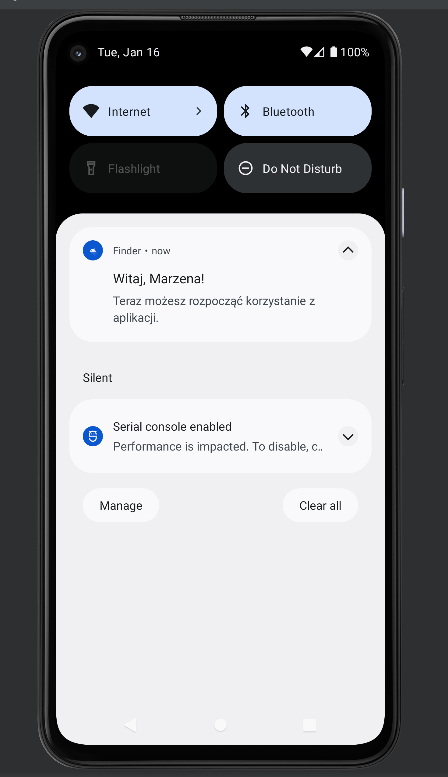
\includegraphics[width=5.5 cm]{rys/pu/3.png}
			\caption{Zmiana imienia-powiadomienie}
			\label{rys:zmiana imienia-powiadomienie}
		\end{center}
	\end{figure}